
%#############################################################################
%
%              						CHAPTER 
%
%#############################################################################
%title old : Concepts et éléments mathématiques de l'apprentissage profond
%title new : Concepts et état de l'art

\textcolor{cyan}{\chapter{Concepts de base et état de connaissances}\label{chap:concept}}
	%\textcolor{cyan}{\chapter{Les bases mathématiques pour l'apprentissage automatique }}%Machine Learning
	\section{Les Éléments d'optimisation numérique} \label{sec:optimisation}
		%\subsection{Éléments de calcul différentiel}\label{sec:diffierential}
		%Cette section est inspirée des notes écrites par le Professeur TSHIMANGA \cite[voir][page:45-82]{jtshiman:2021} et d'autres consignes données par Nocedal et al dans \cite{bottou2018optimization} \cite{coulombeau2013math}[??].
		\subsection{Convexité} \label{subsec:convex}
		%\paragraph*{Ensemble convexe} 
		%Une partie $ {C} \subset \mathbb{R}^n $ est dite convexe si et seulement si pour tout $(x,y) \in {C}^2$, et pour tout $ \alpha \in [0, 1]$, $ \alpha x + (1 - \alpha)y \in \mathcal{C}$ combinaison convexe \cite{jtshiman:2021}.
		\begin{wrapfigure}{r}{0.4\textwidth}
			\myfloatalign{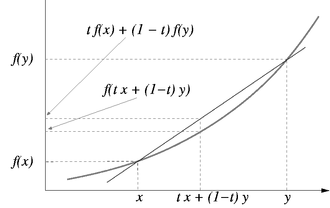
\includegraphics[width=7cm]{images/convex_function_graph-2}}
			\caption[Illustration d'une fonction convexe]{Une fonction convexe, ici $\alpha=t$. }
			\label{fig:convexe_graph}
		\end{wrapfigure}
		La notion de convexité est important lorsque nous voulons minimiser une fonction.
		Autrement dit, une fonction convexe fait référence à une fonction dont le graphique a la forme d'une tasse $\bigcup$ ou une forme incurvée (Comme l'illustre la figure \ref{fig:convexe_graph}).
		
		%\paragraph*{Fonction convexe}
		De manière équivalente, une fonction est convexe si et seulement si la région (ou ensemble des points) au-dessus de son graphe est un ensemble convexe ${C}$ \cite{coulombeau2013math}.\\
		Une fonction $f$ d'un intervalle réel $I \in {C}$ (ensemble convexe) est dite fonction convexe lorsque, $\forall (x,y)$ de $I$ tel que $(x,y) \in {C}^2$ et tout $\alpha \in [0, 1]$, \cite{jtshiman:2021}  on a :
		\begin{equation*}
			\begin{split}
				 f(\alpha x + (1 - \alpha)y) \leq \alpha f(x) + (1 - \alpha)f(y) \\ 
				  et \ si \qquad \qquad \qquad \qquad \\
				 f(\alpha x + (1 - \alpha)y) < \alpha f(x) + (1 - \alpha)f(y) \\
				 \label{eq:convexe}
			\end{split}
		\end{equation*}
		on dit que la fonction est strictement convexe dans ${C}$,  \cite{jtshiman:2021}. Une fonction deux fois différentiable d'une seule variable est convexe si et seulement si sa dérivée seconde est non négative sur tout son domaine \cite{benner2015numerical}.
		%Exemple: 
		%\begin{itemize}
		%\item[--] La fonction $ f(x) = x^2$ est convexe. 
		%\item[--] La fonction $ f(x) = x^T x$ est convexe.
		%\item[--] La fonction $ f(x) = x^T Ax$ est convexe, ssi A est symétrique semi-définie %positive.
		%\end{itemize}coulombeau2013math
		
		%\subsection{Extrema}	
		\paragraph*{Extremum d'une fonction \cite{coulombeau2013math}: }
		%Parmi les propriétés de dérivabilité il existe une qui est mise en relation avec l'effect qu'une fonction doit être convexe. 
		%\cite[][p. 212]{coulombeau2013math}
		\begin{list}{+}{Soit $I \rightarrow  \mathbb{R} $ une fonction et $a$ un point de $I$ ($a \in I$).}
			\item  {On dit que $m$ est un \textbf{minimum local} de $f$, si pour tout $x \in I,\ f(x) \leq f(a)$ ou
				s'il existe $\alpha > 0$ tel que $m$ soit le minimum de $f$ restreinte à $I \cap ] a-\alpha, a + \alpha [$. }
			\item On dit que $M$ est un \textbf{maximum local} de $f$, si pour tout $x \in I,\ f(x) \geq f(a)$ ou s'il existe $\alpha > 0$ tel que $M$ soit le maximum de $f$ restreinte à $I \cap ] a-\alpha, a + \alpha [$. 
		\end{list}
		
		Donc nous pouvons dire qu'une fonction convexe à un unique point minimum. Les fonctions convexes sont, avec les ensembles convexes, jouent aussi un rôle singulier en optimisation, en supprimant la distinction entre minima locaux et globaux, tout minimum local d'une fonction convexe est un minimum global \cite{coulombeau2013math}.
		La fonction carré et la fonction exponentielle sont des exemples de fonctions strictement convexes sur l'ensemble réel $\mathbb {R} $.
		
		Cette notion nous sera plus utile lorsque nous voudrions minimiser notre fonction coût.  
		
		\subsection{{Gradient}}\label{sec:gradient}
		%\paragraph*{Définition:}
		Minimiser une fonction consiste à trouver sa valeur minimum. La valeur minimum d'une fonction se trouve lorsque sa dérivée s'annule en un point de son ensemble de définition et change de signe passant de négatif à positif \cite{coulombeau2013math}. Pour les fonctions scalaires à variables vectorielles on utilise le gradient à la place du dérivé \cite{jtshiman:2021}.\\
		%Le \textbf{gradient} d'une fonction de plusieurs variables (c.a.d à variables vectorielles) en un certain point est un vecteur qui caractérise la variabilité de cette fonction au voisinage de ce point. 
		Le gradient est la généralisation à plusieurs variables de la dérivée d'une fonction d'une seule variable \cite{benner2015numerical, bierlaire2006introduction}.%\\ \\
		%\paragraph*{Définition mathématique :} 
		
		Dans un système de coordonnées cartésiennes, le gradient d'une fonction {$ f(x_{1},x_{2},\dots ,x_{n}$)} est le vecteur de composantes {$ \partial f/ \partial x_{i}\ (i=1,2,\dots ,n)$}, c'est-à-dire les dérivées partielles de $f$ par rapport aux coordonnées \cite{jtshiman:2021}.
		
		\begin{equation}
			{\nabla f(x)={
					\begin{bmatrix}
					{\frac {\partial f(x)}{\partial x_{1}}}\\
					\vdots \\
					{\frac {\partial f(x)}{\partial x_{n}}}
					\end{bmatrix}}} \in \mathbb{R}^n 
		\end{equation}
		
		%\pagebreak
		%\paragraph*{Gradient sous forme de développement limité:}
		%\textit{Si une application admet un gradient en un point, alors on peut écrire ce développement limité du premier ordre. %(voir le point \ref{sec:dev_lim}, équation \ref{eq:dev_lim_h} et \ref{eq:dev_lim_cont})
		%}.
		
		%$${f(x+h)=f(x)+\langle \nabla f(x)\mid h\rangle +o(h) }$$ 
		%ou 
		%$$ {f(x-h)=f(x)-\langle \nabla f(x)\mid h\rangle +o(h)}$$
		%\textit{Numériquement, il est très intéressant de faire ensuite la demi-différence des deux développements pour obtenir la valeur du gradient et on note que celui-ci ne dépend pas en fait de la valeur de la fonction au point $x : f (x)$. Cette formule a l'avantage de tenir compte des gradients du 2e ordre et est donc beaucoup plus précise et numériquement robuste \cite{jtshiman:2021}. L'hypothèse est, en pratique, de connaitre les valeurs "passé" et "futur" de la fonction autour d'un petit voisinage du point $x$} \cite{bierlaire2006introduction}.\\
		%\paragraph*{Définition numérique:}
		Une fonction multivariée, à variable vectorielle, $ f(x)	: \mathbb{R}^n \rightarrow \mathbb{R} : x \rightarrow f(x) $ définie sur ensemble un ouvert $O \in \mathbb{R}^n$ est dite dérivable \cite{jtshiman:2021} en $x$ ssi il existe un vecteur noté $\nabla f(x) \in \mathbb{R}^n$ tel que
		\begin{equation}
		f(x+h) = f(x) + \nabla f(x)^{T}h + o(||h||)
		\end{equation}
		
		avec $\nabla f(x) \in \mathbb{R}^n$ et où l’on a posé que le reste $o(||h||) = ||h||\epsilon (h) \in \mathbb{R}^n$, avec $h \in \mathbb{R}^n$ 
		\begin{equation*}
			\epsilon (h): \mathbb{R}^n\rightarrow \mathbb{R}, \qquad \lim\limits_{||h|| \rightarrow 0} \epsilon(h)=0
		\end{equation*} 
		Le vecteur $\nabla f(x)$ est unique et nommé {gradient} de $f(x)$ en $x$.
		Le gradient s’adresse aux fonctions scalaires à variables vectorielles.
		%\paragraph*{A propos de la notation \textbf{$o(||h||)$}:}
		%La notation de Bachmann-Landau $o(||h||)$ traduit le comportement d’une fonction de $h$ qui tend vers $0$ d’un ordre de grandeur plus vite que $||h||$ \cite{coulombeau2013math}. Elle est infiniment plus petit que $h$ dans le voisinage de $0$.
		

	
	
	%#############################################################################
	%           	SECTION MODELE 
	%#############################################################################
	
	
	%\textcolor{cyan}{\chapter{Apprentissage automatique : Modélisation et Classification }}
	%\section{Généralité}
	
	\section{Concepts de la modélisation et classification des données}
	%\subsection{Introduction} \label{sec:intro_model}
	
	\subsection{{Concepts de la modélisation}}\label{subsec:modelisation}
	La modélisation est la conception et l'utilisation d'un \textit{modèle}. Selon son objectif et les moyens utilisés, la modélisation est dite mathématique, géométrique, 3D, etc. \\
	La modélisation permet de concevoir l'architecture globale d'un système d'information, ainsi que l'organisation des informations à l'aide de la modélisation des données \cite{matloff2017statistical}.
	
	%\paragraph*{Modèle:} 
	Dans notre contexte nos modèle sont mathématique. Un \textbf{modèle mathématique} est une description d'un système utilisant des concepts et un langage mathématiques \cite{darlington2016regression}.\\
	Ce modèle peut aider à expliquer un système et à étudier les effets de différents composants, et à faire des prédictions sur le comportement \cite{harrell2001regression}.
	
	%\paragraph*{Modèle (informatique):} 
	%\textordfeminine\textordfeminineEn informatique, un modèle a pour objectif de structurer les informations et activités d'une organisation : données, traitements, et flux d'informations entre entités \cite{darlington2016regression, matloff2017statistical}.
	
	\subsubsection{\textbf{Modèles non paramétriques}} \label{subsec:modelisation-param}
	
	
	%\Eg: Prenons l'exemple de données décrites dans l'espace d'entrée $\mathcal{X} = \mathbb{R}^n$ avec $n$ variables réelles et supposons-les étiquetées par $\times$ ou par $\textasteriskcentered$. On cherche donc une fonction de décision $h$, appelée hypothèse ou modèle, telle qu'elle soit capable d'étiqueter toute entrée 
	%$x \in \mathcal{X}, h: x \rightarrow \{\times,\textasteriskcentered\}$. Reste à définir l'espace des hypothèses ou modèles $\mathcal{H}$ que l'on est prêt à considérer.
	
	%Toujours en considérant le problème de prédiction basique (présenté ci-dessus), on pourrait définir une hypothèse par une procédure qui examine les trois plus proches voisins du point à étiqueter $x$ et qui choisit l'étiquette majoritaire parmi ces trois points pour étiqueter $x$. Il n'y a évidemment plus de paramètres pour définir les modèles possibles \cite{antoine2018apprentissage}.
	
	Un {modèle non paramétrique} est construit selon les informations provenant des données. Dans \cite{bishop2006pattern, antoine2018apprentissage} il est expliqué que : La régression non paramétrique exige des tailles d'échantillons plus importantes que celles de la régression basée sur des modèles paramétriques parce que les données doivent fournir la structure du modèle ainsi que les estimations du modèle.
	
	Un {modèle paramétrique} est, s'il est approximativement valide, plus puissant qu'un modèle non paramétrique, produisant des estimations d'une fonction de régression qui ont tendance à être plus précises que ce que nous donne l'approche non paramétrique \cite{matloff2017statistical}. Cela devrait également se traduire par une prédiction plus précise. 
	
	
	\begin{list}{--}{Dans \cite{antoine2018apprentissage}, il est expliqué que nous pouvons construire un modèle d'apprentissage, ou l'espaces des hypothèses d'apprentissage, par: }
		\item La classification
		\item La régression
		\item Les distributions de probabilités
		\item Les arbres de décisions
		\item Les réseaux bayésiens 
		\item Etc.
	\end{list}	
	
	\subsubsection{\textbf{Entraînement du modèle}}
	
	Tout modèle, où toutes les informations nécessaires ne sont pas disponibles, contient certains paramètres qui peuvent être utilisés pour adapter le modèle au système qu'il est censé décrire. Si la modélisation est effectuée par un réseau de neurones artificiels ou un autre apprentissage automatique, l'optimisation des paramètres est appelée \textbf{entraînement} (en anglais : \textbf{training}), tandis que l'optimisation des hyperparamètres du modèle est appelée \textbf{réglage} (en anglais: \textbf{tuning}) et utilise souvent la validation croisée \cite{goodfellow2016deep}. Dans une modélisation plus conventionnelle à travers des fonctions mathématiques explicitement données, les paramètres sont souvent déterminés par ajustement de courbe (voir le chapitre \ref{chap:methode}, section \ref{sec:desc_grad}).
	
	Une partie cruciale du processus de modélisation consiste à évaluer si oui ou non un modèle mathématique donné décrit un système avec précision. Il peut être difficile de répondre à cette question car elle implique plusieurs types d'évaluation différents \cite{matloff2017statistical, goodfellow2016deep}.
	
	\subsection{Les problèmes de régressions} \label{sec:regression_problem}
	
	L'algorithme d'apprentissage automatique est défini comme un algorithme capable d'améliorer les performances d'un programme informatique à certaines tâches via l'expérience est quelque peu abstraite. Pour rendre cela plus concret, Une des méthode d'apprentissage automatique basique est \emph{la régression linéaire} \cite{goodfellow2016deep}.
	
	%Dans la modélisation statistique, l'analyse de régression est un ensemble de processus statistiques permettant d'estimer les relations entre une variable dépendante et une ou plusieurs variables indépendantes \cite{matloff2017statistical}.\\
	En statistique, la régression linéaire est une approche linéaire pour modéliser la relation entre une réponse scalaire (\cf$ \ $ section \ref{subsec:modelisation}) et une ou plusieurs variables explicatives (également appelées variables dépendantes et indépendantes). Le cas d'une variable explicative est appelé régression linéaire simple; pour plus d'un, le processus est appelé régression linéaire multiple \cite{darlington2016regression}.
	
	%Dans la régression linéaire, les relations sont modélisées à l'aide de \textit{fonctions prédictives}%\footnote{En apprentissage automatique, une fonction de prédicteur linéaire est une fonction linéaire d'un ensemble de coefficients et de variables explicatives, dont la valeur est utilisée pour prédire le résultat d'une variable dépendante.} 
	%linéaires dont les paramètres de modèle inconnus sont estimés à partir des données \cite{matloff2017statistical}. De tels modèles sont appelés modèles linéaires.
	
	Les problèmes de régressions ont de nombreuses utilisations pratiques. Si l'objectif est la prédiction, la prévision ou la réduction des erreurs, la régression peut être utilisée pour ajuster un modèle prédictif à un ensemble de données observées de valeurs de la réponse et de variables explicatives \cite{darlington2016regression}. Après avoir développé un tel modèle, si des valeurs supplémentaires des variables explicatives sont collectées sans valeur de réponse d'accompagnement, le modèle ajusté peut être utilisé pour faire une prédiction de la réponse \cite{harrell2001regression}.
	
	%Dans ce type de tâche, le programme informatique est invité à prédire une valeur numérique à partir d'une entrée donnée. Pour résoudre cette tâche, l'algorithme d'apprentissage est invité à sortir une fonction $f : \mathbb{R}^n \rightarrow \mathbb{R}$. Ce type de tâche est similaire à la \textbf{classification}, sauf que le format de sortie est différent  \cite{goodfellow2016deep}.
	
	\subsubsection{Le cas de la régression générale}
	La plupart des modèles de régression proposent que $Y_{i}$ est une fonction de $X_{i}$ et $w$, avec $\epsilon_{i}$ représentant un terme d'erreur additif ou bruit statistique aléatoire qui peut remplacer des déterminants non modélisés de $Y_{i}$ :
	\begin{equation}
	{\displaystyle Y_{i}=f(X_{i},w )+\epsilon_{i}}
	\end{equation}
	
	L'objectif est d'estimer la fonction ${\displaystyle f(X_{i},w )}$ qui correspond le mieux aux données.\\
	Pour effectuer une analyse de régression, la forme de la fonction $f$ doit être spécifié. Parfois, la forme de cette fonction est basée sur l'information de la relation entre $Y_{i}$ et $X_{i}$. 
	Si ces informations ne sont pas disponibles, un cas souple ou pratique pour $f$ est choisi. Par exemple, une simple régression univariée peut proposer
	$${\displaystyle f(X_{i},w )= w_{0}+ w_{1}X_{i}}$$
	ou
	$${\displaystyle Y_{i}= w_{0}+ w_{1}X_{i}+e_{i}}$$
	être une approximation raisonnable du processus statistique générant les données.
	
	Différentes formes d'analyse de régression fournissent des outils pour estimer les paramètres. $w$. Par exemple, les moindres carrés trouvent la valeur de $w$ qui minimise la somme des carrés des erreurs \cite{deepa2021ai}. $${\sum _{i}^n (Y_{i}-f(X_{i},w ))^{2}}$$ 
	
	Étant donné un ensemble de données ${\displaystyle \{y_{i},\,x_{i1},\ldots ,x_{ip}\}_{i=1}^{n}}$ de $n$ unités statistiques, un modèle de régression linéaire suppose que la relation entre la variable dépendante $y$ et le vecteur $w$ des régresseurs $x$ est linéaire. Cette relation est \textbf{modélisée} par un terme de perturbation ou une variable d'erreur $\epsilon$ : une variable aléatoire non observée qui ajoute du "bruit" à la relation linéaire entre la variable dépendante et les régresseurs \cite{antoine2018apprentissage, darlington2016regression}. Ainsi le modèle prend la forme
	
	$${\displaystyle y_{i}=w _{0}+w _{1}x_{i1}+\cdots +w _{n}x_{in}+\varepsilon _{i}=\mathbf { x} _{i}^{\mathsf {T}}{\boldsymbol {w }}+\varepsilon_{i},\qquad avec \quad i=1,\ldots ,n,}
	$$
	
	Souvent, ces $n$ équations sont empilées et écrites en notation matricielle comme
	
	\begin{equation}\label{eq:regression_generale}
		{\displaystyle \mathbf {y} =X{\boldsymbol {w}}+{\boldsymbol {\varepsilon}},\,}
	\end{equation}
	

	
	où
	
	$
	\mathbf{y} ={\begin{pmatrix}y_{1}\\y_{2}\\\vdots \\y_{n}\end{pmatrix}},\quad
	{\displaystyle 
		X={
			\begin{pmatrix}
			\mathbf {x} _{1}^{\mathsf {T}}\\
			\mathbf {x} _{2}^{\mathsf {T}}\\
			\vdots \\
			\mathbf {x} _{n}^{\mathsf {T}}
			\end{pmatrix}}={
			\begin{pmatrix}
			1&x_{11}&\cdots &x_{1p}\\
			1&x_{21} &\cdots &x_{2p}\\
			\vdots &\vdots &\ddots &\vdots \\
			1&x_{n1}&\cdots &x_{np}
			\end{pmatrix}},} \quad
	{\displaystyle {\boldsymbol {\boldsymbol{w}}}={
			\begin{pmatrix}
			w _{0}\\
			w _{1}\\
			w _{2}\\
			\vdots \\
			w _{p}
			\end{pmatrix}},\quad 
		{\boldsymbol {\varepsilon }}={
			\begin{pmatrix}\varepsilon _{1}\\
			\varepsilon _{2}\\
			\vdots \\
			\varepsilon _{ n}
			\end{pmatrix}}.}$ \\
	
	$\mathbf{y}$ est un vecteur de valeurs observées ${\displaystyle y_{i}\ (i=1,\ldots ,n)}$ de la variable appelée variable mesurée ou variable dépendante.
	
	$X$ peut être vu comme une matrice de vecteurs-lignes $\mathbf {x} _{i}$ ou de vecteurs-colonnes à $n$ dimensions $X_{j}$, appelées régresseurs, variables explicatives, variables d'entrée, variables prédictives ou variables indépendantes. La matrice $X$ est parfois appelée la matrice de conception. 
	
	${\boldsymbol {w}}$ est un vecteur de paramètre de dimension $(p+1)$, où $w _{0}$ est le terme d'interception, s'il n'est pas inclus dans le modèle ${\boldsymbol {w}}$ est de dimension $p$. Ses éléments sont appelés coefficients de régression \cite{antoine2018apprentissage}. 
	En régression linéaire simple, $p = 1$, et le coefficient est appelé \textbf{pente} de régression.
	
	
	L'estimation statistique et l'inférence dans la régression linéaire se concentrent sur $w$. Les éléments de ce vecteur de paramètres sont interprétés comme les dérivées partielles de la variable dépendante par rapport aux différentes variables indépendantes \cite{darlington2016regression}.
	
	En définissant les vecteurs  et matrice ci dessous, ${\boldsymbol X}$, ${\boldsymbol w}$ et ${\boldsymbol y}$ (avec ${S_y = y}$) \cite{antoine2018apprentissage}; le critère de la somme des carrées des erreurs s'écrit alors:
	\begin{equation}\label{eq:sce_2}
	SCE(w|\mathit{S}) = \frac{1}{2} ({\boldsymbol S_y }- \mathbf{X}\boldsymbol w)^{\mathsf{T}}({ \boldsymbol S_y }- \mathbf{X} \boldsymbol w)
	\end{equation}  
	Il suffit de prendre la dérivée de la somme des carrés des erreurs (équation \ref{eq:sce_1}) par rapport à $w$, qui est maintenant remplacer par $w$, pour obtenir les équations: 
	$$
	\frac{\partial SCE}{\partial w} = -{\boldsymbol X}^T({\boldsymbol S_y }- \mathbf{X} \boldsymbol w)
	$$
	
	$$
	\frac{\partial^2 SCE}{\partial^2 w \partial^2 w^T} = -{\boldsymbol X}^T{\boldsymbol X}
	$$
	
	En supposant que la matrice $X$ est non singulière, et donc que $X^TX$ est positive définie, et en posant que la dérivée première est nulle, on obtient :
	\begin{equation}
	{X^{T} Xw =  X^{T} S_y}
	\end{equation}
	à partir de quoi on peut calculer l'unique solution par: 
	\begin{equation}
	\hat{w} = {(X^{T} X)^{-1} X^{T} S_y}
	\end{equation}
	La valeur $\hat{y}$ prédite pour une entrée $x_n$ est donc : 
	$$
	\hat{y} = \hat{w}\cdot x_n = {(X^{T} X)^{-1} X^{T} S_y}x_n 
	$$ 
	
	
	%Un modèle de régression linéaire ajusté peut être utilisé pour identifier la relation entre une seule variable prédictive $x_j$ et la variable de réponse $y$ lorsque toutes les autres variables prédictives du modèle sont "maintenues fixes". Plus précisément, l'interprétation de $\beta_j$ est la variation attendue de $y$ pour une variation d'une unité de $x_j$ lorsque les autres covariables sont maintenues fixes, c'est-à-dire la valeur attendue de la dérivée partielle de $y$ par rapport à $x_j$. Ceci est parfois appelé l'effet unique de $x_j$ sur $y$. En revanche, l'effet marginal de $x_j$ sur $y$ peut être évalué à l'aide d'un coefficient de corrélation ou d'un simple modèle de régression linéaire reliant uniquement $x_j$ à $y$; cet effet est la dérivée totale de $y$ par rapport à $x_j$.
	
	%\subsection{La régression linéaire simple}
	%\lipsum[3]
	%\subsection{La régression linéaire multivarié}
	%\subsubsection{Droite de régression} 
	%\subsubsection{Variance, Covariance, \& Corrélation}
	%\subsection{La fonction prédictif \& d'erreur}
	%\lipsum[1]
	
	%\begin{figure}[H]%bth
		%\centering
		%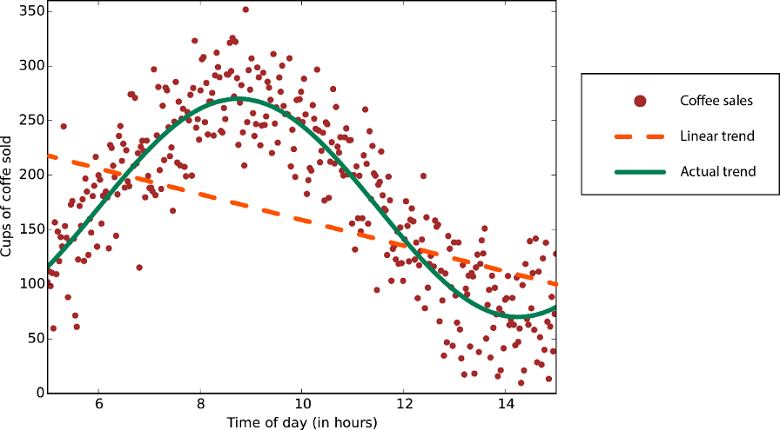
\includegraphics[width=\textwidth]{images/nonlinear-trend.png}
		%\caption{ L'efficacité de la régression non linéaire par rapport \`{a} une régression linéaire..}
		%\label{fig:nonlinear_trend}
	%\end{figure}
	
	\paragraph*{régression linéaire multiple}
	La régression linéaire multiple est une généralisation de la régression linéaire simple au cas de plus d'une variable indépendante, et un cas particulier des modèles linéaires généraux, limités à une variable dépendante.
	
	
	\subsection{Les problèmes de classifications} \label{sec:classificarion_problem}
	En apprentissage automatique, les classifieurs linéaires sont une famille d'algorithmes de classement statistique. Le rôle d'un classifieur est de classer dans des groupes (des classes) les échantillons qui ont des propriétés similaires, mesurées sur des observations. Un classifieur linéaire est un type particulier de classifieur, qui calcule la décision par combinaison linéaire des échantillons \cite{antoine2018apprentissage}.
	
	\begin{figure}[bth]%bth
		\centering
		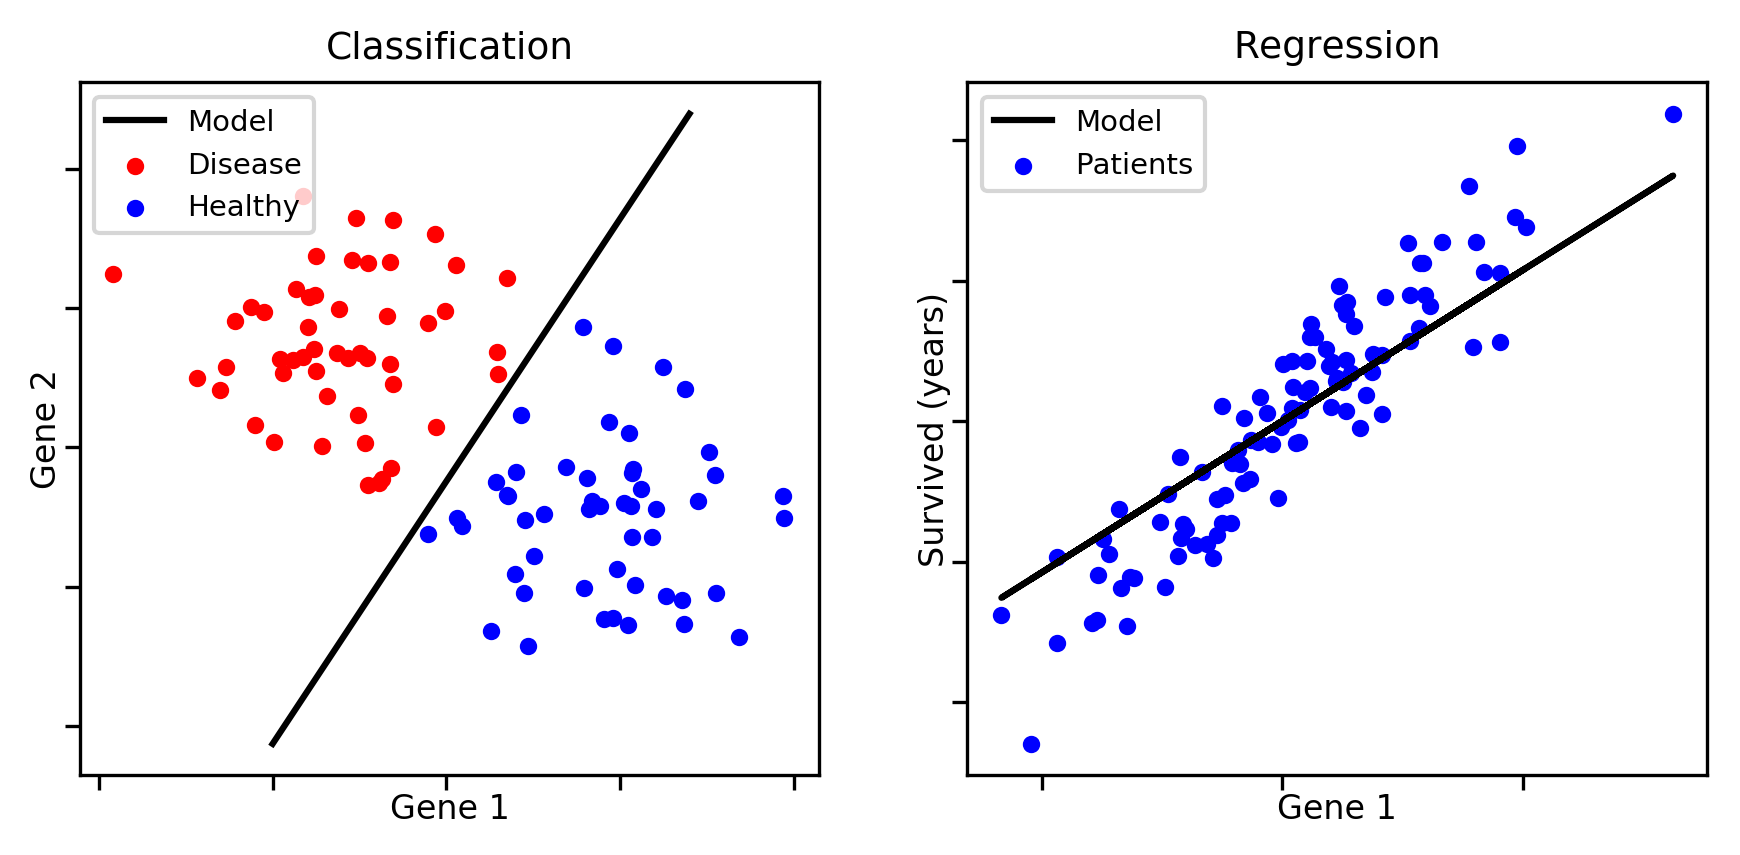
\includegraphics[width=15cm]{images/classification_vs_regression.png}
		\caption[Classification vs Régression.]{Classification vs régression \cite{ml2008python}.}
		\label{fig:class_vs_reg}
	\end{figure}
	
	Nous nous plaçons dans le cadre où la variable dépendante ou à prédire prend ses valeurs dans un ensemble fini que l'on associe généralement à un ensemble de classes. A la différence de la régression linéaire où l’ensemble de valeurs à prédire est infini.
	
	Lorsque l'on se place dans un espace de représentation euclidien, on peut librement faire des hypothèses sur la géométrie des classes ou sur celles de leurs surfaces séparatrices. La plus simple d'entre elles est de supposer que deux classes peuvent être séparées par une certaine surface, définie par une équation; les paramètres qui régissent cette équation sont alors les variables à apprendre.
	
	Le nombre de paramètres à calculer est minimal si l'on suppose cette surface linéaire; aussi est-ce l'hypothèse qui prévaut souvent, en particulier lorsque l'échantillon de données est de taille réduite par rapport à la dimension de l'espace d'entrée, d'autant qu'elle permet de mener des calculs faciles et de visualiser précisément le résultat obtenu \cite{sarkar2017practical}.
	
	Dans $\mathbb{R}^n$, une surface linéaire est un hyperplan $A$, défini par l'équation :
	$$ 
	a_0  + a^Tx = 0
	$$
	
	avec $a$ vecteur de dimension $n$ et $a_0$ scalaire. Si deux classes $\mathcal{C}_1$ et $\mathcal{C}_2$ sont \textit{séparables} par $A$, tous les points de la première classe sont par exemple tels que :
	
	\begin{equation}\label{eq:x_case_c1}
	x \in \mathcal{C}_1 \implies a_0 + a^Tx > 0
	\end{equation}
	
	et ceux de la seconde vérifient alors :
	
	\begin{equation}\label{eq:x_case_c2}
	x \in \mathcal{C}_2 \implies a_0 + a^Tx \leq 0
	\end{equation}
	
	
	Dans un espace de dimension $d = 1$, une séparation linéaire se réduit à la comparaison à un seuil. Prenons ce cas particulier pour donner deux exemples où un problème de discrimination à deux classes ne peut pas en pratique être complètement résolu par une séparatrice linéaire.
	
	\paragraph* {séparatrice linéaire :}On appelle hyperplan séparateur ou séparatrice linéaire un hyperplan qui sépare parfaitement deux classes, c'est-à-dire qui vérifie les équations \ref{eq:x_case_c1} et \ref{eq:x_case_c2}; en particulier, il sépare parfaitement leurs points d'apprentissage. Un hyperplan discriminant est un classificateur linéaire pour deux classes qui ne sont pas linéairement séparables \cite{antoine2018apprentissage}.
	
	%\subsubsection{Le cas non séparable}
	\begin{figure}[H]%bth
		\centering
		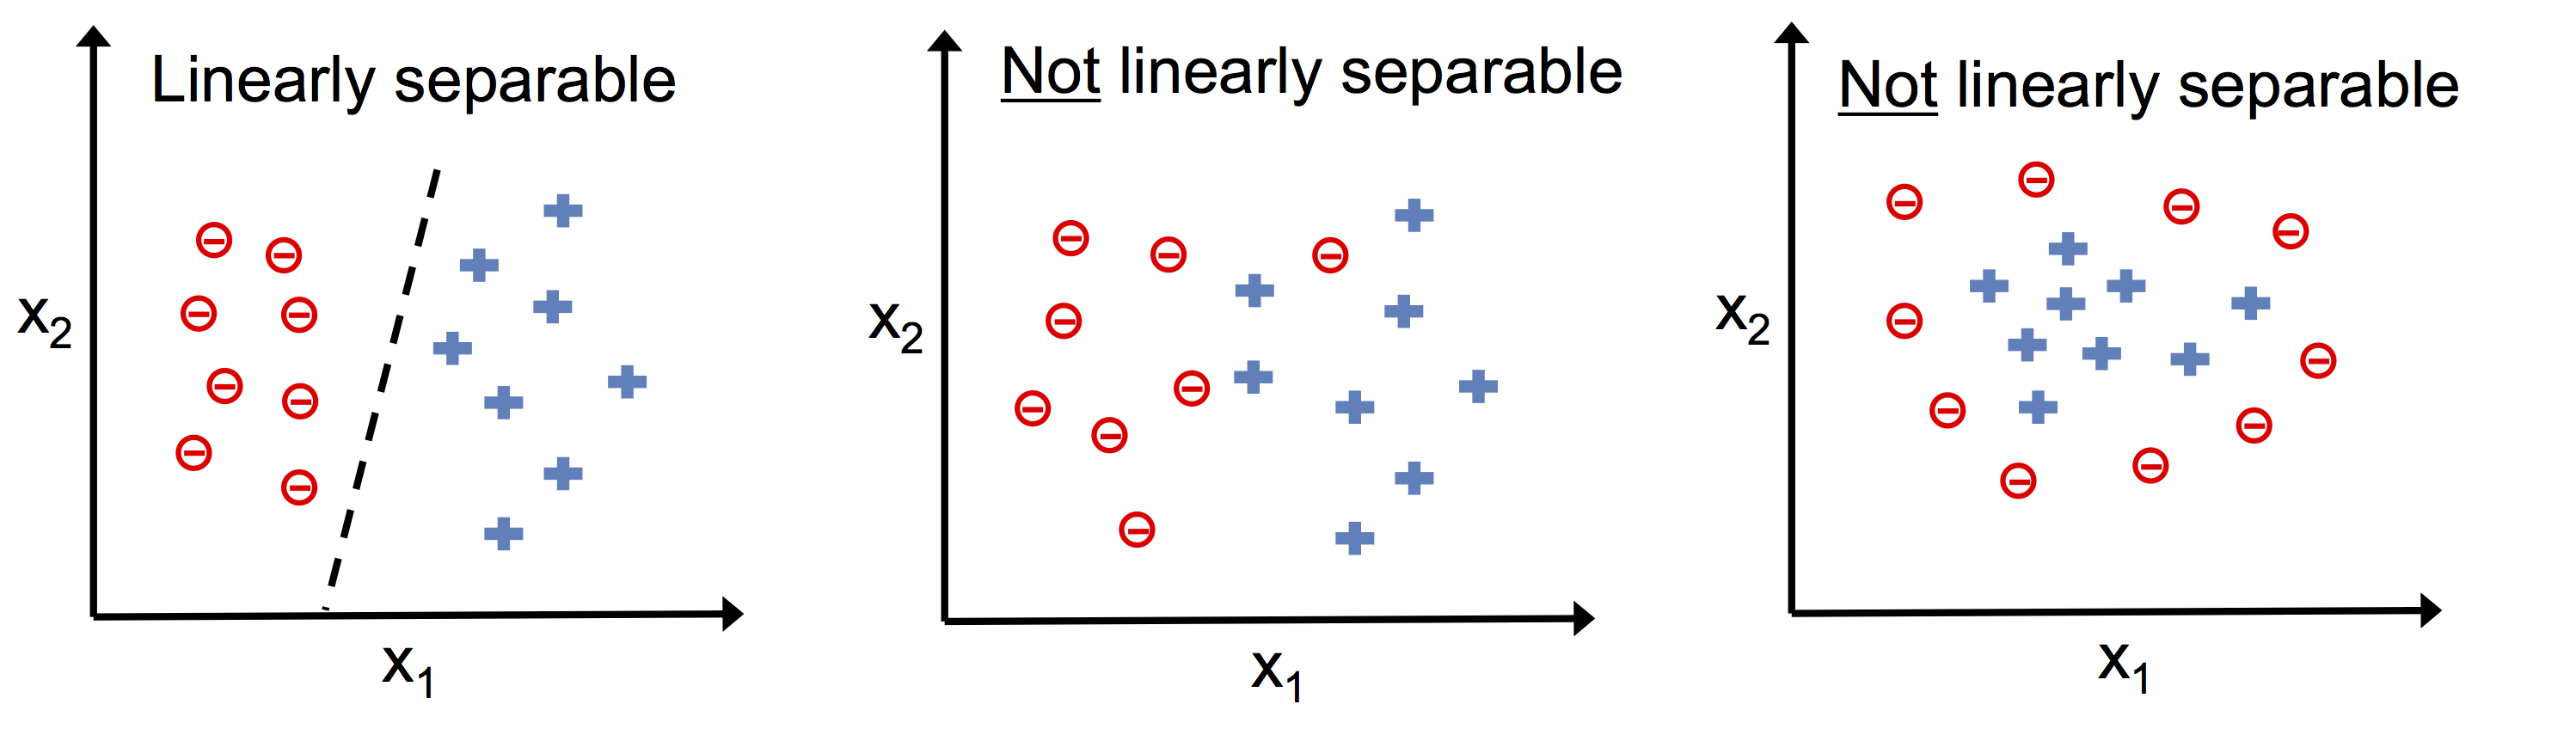
\includegraphics[width=\textwidth]{images/linearly_separable.png}
		\caption[Classes linéairement séparables.]{Classes linéairement séparables \cite{ml2008python}}
		\label{fig:linearly_separable}
	\end{figure}
	
	
	
	\subsubsection{Le modèle de la régression logistique} \label{subsec:reg_logistique}
	
	\begin{wrapfigure}{r}{0.3\textwidth}
		\myfloatalign{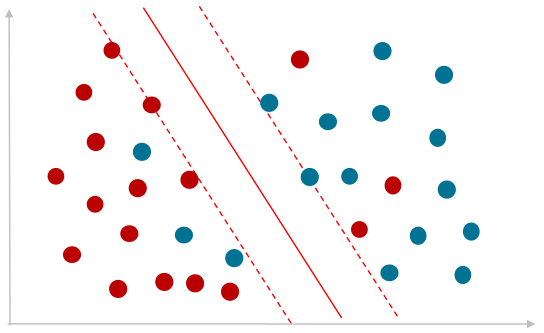
\includegraphics[width=6cm]{images/classification_minimisation}}
		\caption{Droite séparatrice.}\label{fig:classification_2case}
	\end{wrapfigure}
	Ce qu'il est convenu d'appeler \textit{régression logistique} concerne en fait une méthode de classification binaire. 
	%à l'instar du perceptron (voir la section \ref{sec:perceptron}). 
	A la différence du perceptron, cependant, nous allons chercher à apprendre une hypothèse $h$ définie de $\mathbb{R}^n$ dans [0,1], et non pas dans {0,1},  une motivation étant d'interpréter $h(x)$ comme étant la probabilité que l'entrée $x$ appartienne à la classe d'intérêt que nous notons $\mathcal{C}_1$. \cite{antoine2018apprentissage}
	
	La fonction de la droite séparatrice comme l'illustre la figure \ref{fig:classification_2case} s'écrit:
	\begin{equation}\label{eq:droite_sep}
	z = w _{1}x_{1}+\cdots +w_{n}x_{n}+b
	\end{equation}
	
	avec $ i=1,\ldots ,n,$ et $w_i$ et $b$ des paramètres de la droite.  %et $b = \varepsilon$
	\\
	$
	\begin{cases}
	\hat{y}=0 \ \ (y \in \mathcal{C}_1) & \quad \text{si  } z < 0\\
	\hat{y}=1 \ \ (y \in \mathcal{C}_2) & \quad \text{si  } z \geq 0
	\end{cases}
	$\\
	%??? changement de plan
	
	La fonction logistique est une fonction sigmoïde , qui prend n'importe quelle entrée réelle $t$, et renvoie une valeur comprise entre zéro et un \cite{ml2008python}. La fonction logistique standard ${\displaystyle \sigma :\mathbb {R} \rightarrow (0,1)}$ est défini comme suit :
	\begin{equation} \label{eq:sigmoid-simple}
	\sigma (t)={\frac {e^{t}}{e^{t}+1}}={\frac {1}{1+e^{-t}}}
	\end{equation}
	
	Supposons que $t$ est une fonction linéaire (comme la droite de la formule \ref{eq:droite_sep}) $t = z$. Et la fonction logistique générale ${ p:\mathbb {R} \rightarrow (0,1)}$ peut maintenant l'écrire :
	\begin{equation}\label{eq:sigmoid-dev}
	{\displaystyle p(x)=\sigma (z)= {\frac {1}{1+e^{-z}}} ={\frac {1}{1+e^{-(w _{1}x_{1}+\cdots +w_{n}x_{n}+b)}}}}
	\end{equation} 
	
	
	
	Dans le modèle logistique, $p(x)$ est interprété comme la probabilité de la variable dépendante ${Y}$ équivalant à un succès/cas-oui plutôt qu'à un échec/non-cas. Il est clair que les variables de réponse $Y_{i}$ ne sont pas identiquement répartis :$P(Y_{i}=1\mid X)$ diffère d'un point de données $X_{i}$ à l'autre, bien qu'ils soient indépendants étant donné la matrice de conception $X$ et paramètres partagés $w$ \cite{antoine2018apprentissage}. 
	
	
	\begin{figure}[H]%bth
		\centering
		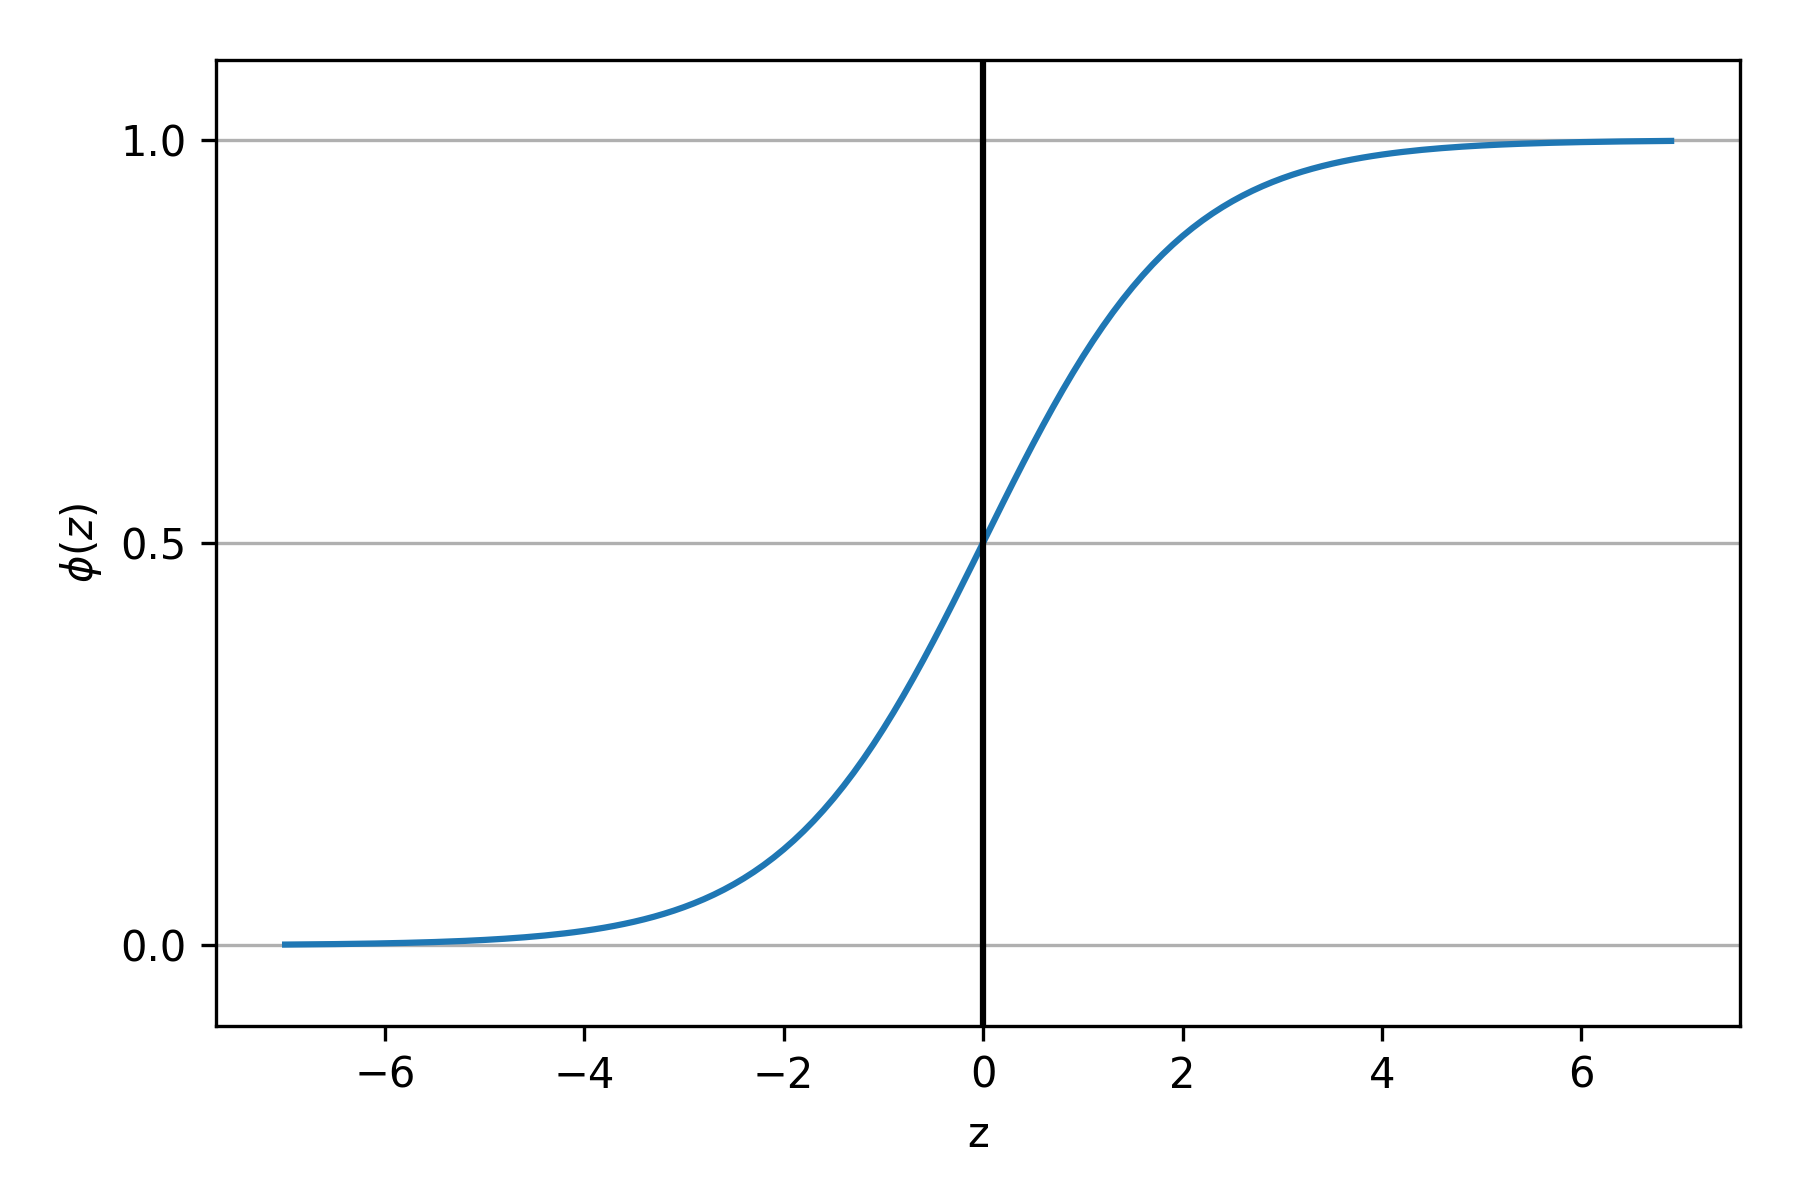
\includegraphics[width=7cm]{images/reg_log_curve.png}
		\caption[Graphique représentant fonction logistique.]{Graphique représentant fonction sigmoïde logistique ajustée aux données $(x_n , y_n)$ \cite{ml2008python}}.
		\label{fig:reg_log_sigmoid}
	\end{figure}
	
	\paragraph*{La vraisemblance:}Indique la plausibilité du  modèle vis-a-vis du vraies données.
	Soit l'échantillon $ \mathcal{S} = {(\mathbf{x}_1, y_1),..., (\mathbf{x}_m, y_m)}$, avec $y_i \in \{\mathcal{C}_1,\mathcal{C}_2\}, \forall_i \in (1,...,m)$. Sa vrai semblance en fonction des paramètres à apprendre s'écrit:
	
	\begin{equation}\label{eq:likelyhood}
	L = \prod_{i=1}^{m} {p_i}^{y_i} (1-p_i)^{1-y_i}
	\end{equation}
	
	où $m$ est le nombre d'exemples d'apprentissage appartenant à la classe.
	
	%Dans \cite{antoine2018apprentissage}, il est montré que ces paramètres peuvent être obtenus par maximisation de la vraisemblance des paramètres conditionnellement aux exemples. Il a été de plus montré que, sous des conditions très générales \cite{sarkar2017practical}, le maximum de $L$ est unique.
	%La maximisation de la vraisemblance se fait sois en passant par le logarithme, pour obtenir la log-vraisemblance :
	%\begin{equation}
	%\begin{split}
	%\log(L)  & = \log(\prod_{i=1}^{m} {p_i}^{y_i} (1-p_i)^{1-y_i}) \\
	%& =\sum_{i=1}^{m} \log( {p_i}^{y_i}) +\log((1-p_i)^{1-y_i})\\
	%& =\sum_{i=1}^{m} {y_i}\log( {p_i}) +{(1-y_i)}\log(1-p_i)\\
	%\end{split}
	%\end{equation}
	%Comme en Machine Learning on est plus habile à minimiser qu'à maximiser et que maximiser une fonction $f(\cdot)$ consiste à minimiser $-f(\cdot)$ alors la log-vraisemblance s'écrira: 
	Dans \cite{antoine2018apprentissage}, il est montré que ces paramètres peuvent être obtenus par maximisation de la vraisemblance des paramètres conditionnellement aux exemples. Maximiser une fonction $f(\cdot)$ consiste à minimiser $-f(\cdot)$ alors la log-vraisemblance s'écrira:
	\begin{equation}\label{eq:log-likelyhood}
		\mathcal{L} = -\frac{1}{m}\sum_{i=1}^{m} {y_i}\log( {p_i}) +{(1-y_i)}\log(1-p_i)
	\end{equation}
	avec le terme $\frac{1}{m}$ pour augmenter la précision. Avec cette fonction, nous allons maximiser la vraisemblance $L$ en minimisant $-\log(L)$.
	
	La log-vraisemblance négative est égale à la perte logarithmique (Log-loss) sous une distribution de probabilité de Bernoulli \cite{darlington2016regression, antoine2018apprentissage}.
	
	
	
	
	
	
	
	%###############################################################################################
	% SECTION : Réseau de neurones, apprentissage en profondeur
	%##############################################################################################	
	
	
	\section{Réseau de neurones, apprentissage en profondeur}
	
	\subsection{Perceptron} \label{sec:perceptron}
	
	Le perceptron est un modèle simplifié d'un neurone biologique. Alors que la complexité des modèles de neurones biologiques est souvent nécessaire pour bien comprendre le comportement neuronal, la recherche suggère qu'un modèle linéaire de type perceptron peut produire certains comportements observés dans de vrais neurones.
	
	%Un perceptron est donc une unité de réseau neuronal, l'élément de traitement de base, qui effectue certains \textit{calculs} pour détecter des caractéristiques ou une intelligence économique dans les données d'entrée.\\ 
	
	Le perceptron, à l'instar du neurone artificiel classique, est conçu avec un algorithme d'apprentissage supervisé du même nom.\\
	L'algorithme du perceptron proposé par Frank Rosenblatt \cite{antoine2018apprentissage}, basé sur le modèle neuronal MP Neuron (McCulloch-Pitts Neuron), est un algorithme qui apprendrait automatiquement les coefficients de poids optimaux qui sont ensuite multipliés par les caractéristiques d'entrée afin de décider si un neurone se déclenche ou non. Dans le cadre de l'apprentissage supervisé et de la classification, un tel algorithme pourrait alors être utilisé pour prédire si un échantillon appartient à une classe ou à l'autre \cite{ml2008python}.
	\begin{figure}[H]%bth
		\centering
		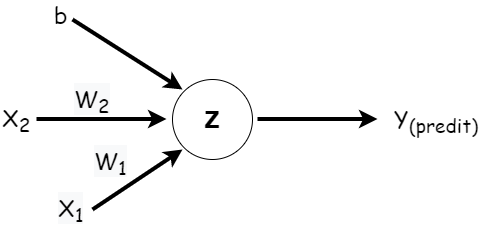
\includegraphics[width=8cm]{images/neuron-3-param.png}
		\caption[Neurone logique avec deux entrées $x_1$ et $x_2$ et les paramètres $w_1$, $w_2$ et $b$.]{Neurone logique avec deux entrées $x_1$ et $x_2$ et les paramètres $w_1$, $w_2$ ($w_i$ dans un réseau de neurones il est nommé poids) et $b$ aussi appelé biais. le fonction d'agrégation $z$ (voir le point \ref{subsec:reg_logistique}, section \ref{sec:regression_problem}  et la formule \ref{eq:droite_sep})  sera: $z=w_1 x_1 +w_2 x_2 + b$.}
		\label{fig:logic_neuron}
	\end{figure}
	
	
	
	Le perceptron a des entrées qui peuvent provenir de l'environnement ou peuvent être les sorties d'autres perceptrons.
	Associé à chaque entrée, $ x_j \in \mathbb{R}$, avec $ j = 1,2, \dots , n, $ est un \textit{poids de connexion, ou poids} synaptique $w_j \in \mathbb{R}$, et la sortie, $\hat{y}$. Dans le cas le plus simple $\hat{y}$ est une somme pondérée des entrées \cite{alpaydin2010introduction}.
	
	$$ {\hat{y} = \sum _{j=1}^{n}w_{j}x_{j} + w_0} $$
	
	$w_0$ est la valeur d'interception pour rendre le modèle plus général, il est généralement modélisé comme la pondération provenant d'une unité de biais supplémentaire, $b = w_0 x_0$, avec $x_0$ qui est toujours égale $+1$. Nous pouvons écrire la sortie du perceptron sous la forme d'un produit scalaire.
	$$ \hat{y} = x^Tw $$
	
	Pendant le test, avec des poids donnés, $w$, pour l'entrée $x$, nous calculons la sortie $\hat{y}$. Pour implémenter une tâche donnée, nous avons besoin d'apprendre les poids $w$, les paramètres du système, de sorte que des sorties correctes soient générées compte tenu des entrées.
	
	\begin{figure}[hth]%bth
		\centering
		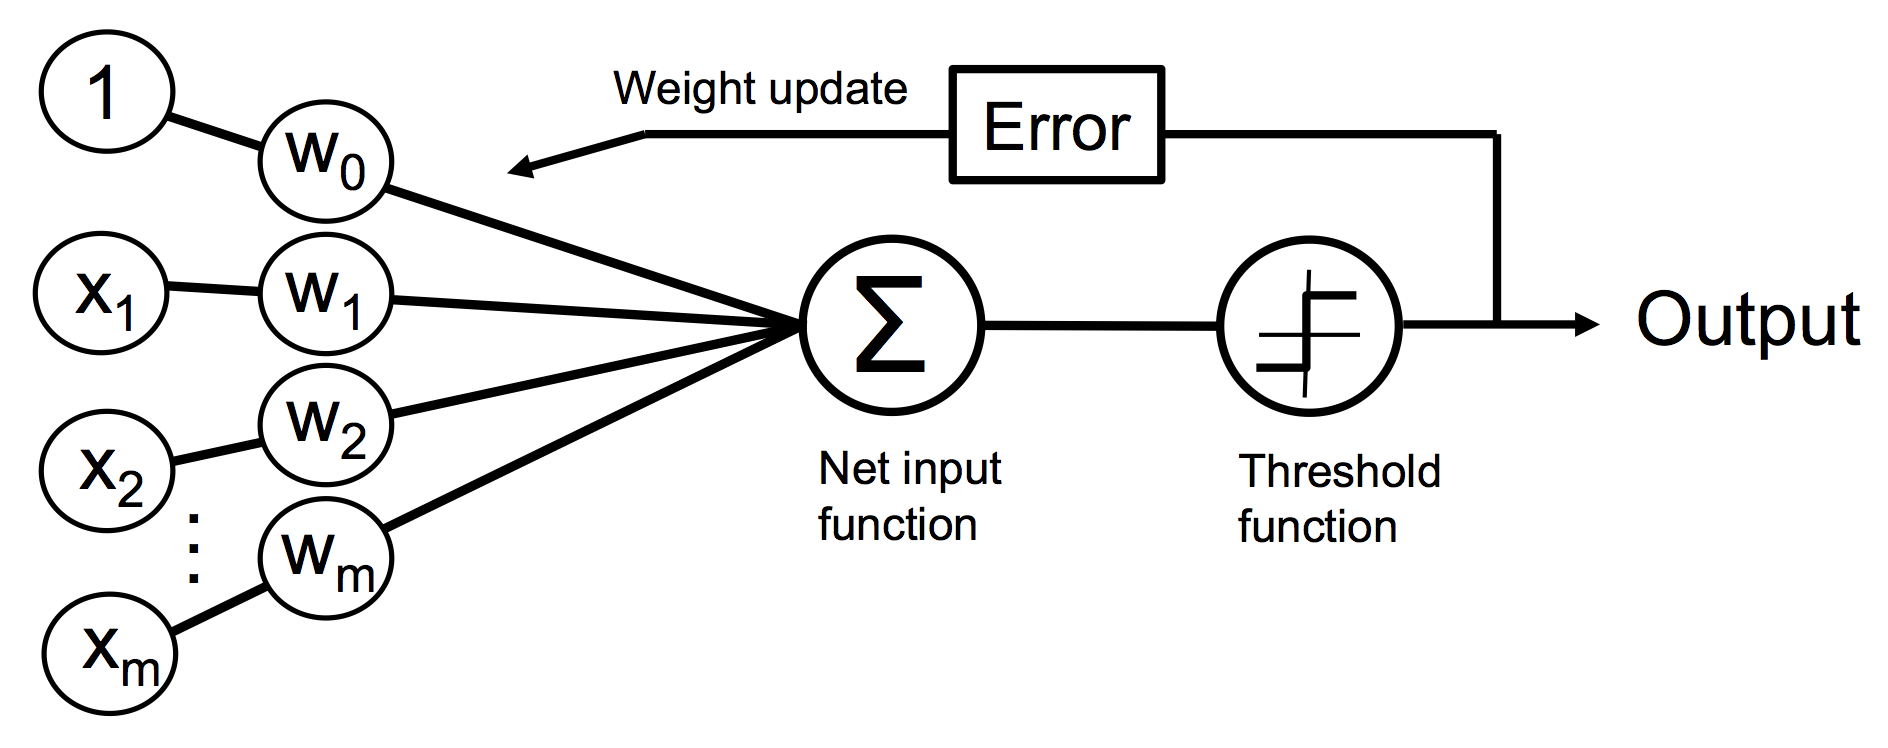
\includegraphics[width=\textwidth]{images/perceptron_neuron.png}
		\caption[Neurone artificiel modèle perceptron.]{Neurone artificiel modèle perceptron \cite{ml2008python}, cette figure est plus adapté pour représenter le modèle du perceptron.}
		\label{fig:perceptron_neuron}
	\end{figure}

	
	
	\subsubsection{Le réseau de neurones artificiels (Perceptron Multicouche)}
	
	Les réseaux de neurones ont été introduits pour la première fois comme méthode d'apprentissage par Frank Rosenblatt, bien que le modèle d'apprentissage appelé perceptron soit différent des réseaux de neurones modernes, nous pouvons toujours considérer le perceptron comme le premier réseau de neurones artificiels \cite{sarkar2017practical}.
	
	Le perceptron multicouche (en anglais: multilayer perceptron MLP) est un type de réseau neuronal artificiel (ANN) organisé en plusieurs couches, où les informations ne circulent que de la couche d'entrée à la couche de sortie. Il s'agit donc d'un réseau à propagation directe (feed forward), autrement dit le réseau profond à action directe. Un perceptron multicouche est juste une fonction mathématique mappant un ensemble de valeurs d'entrée à des valeurs de sortie. La fonction est formée en composant de nombreuses fonctions plus simples. Nous pouvons considérer chaque application d'une fonction mathématique différente comme fournissant une nouvelle représentation de l'entrée \cite{goodfellow2016deep,antoine2018apprentissage}.
	
	Les perceptrons à une seule couche ne sont capables d'apprendre que des motifs linéairement séparables. Pour une tâche de classification avec une \textbf{fonction d'activation} d'étape, un seul nœud aura une seule ligne divisant les points de données formant les motifs. Plus de nœuds peuvent créer plus de lignes de division, mais ces lignes doivent en quelque sorte être combinées pour former des classifications plus complexes. Une deuxième couche de perceptrons, voire de nœuds linéaires, suffit à résoudre de nombreux problèmes autrement non séparables \cite{antoine2018apprentissage}.
	
	Les réseaux de neurones artificiels fonctionnent vaguement sur le principe de l'apprentissage d'une distribution distribuée de données.
	%L'hypothèse sous-jacente est que les données générées sont le résultat d'une combinaison non linéaire d'un ensemble de facteurs latents et si nous sommes capables d'apprendre cette représentation distribuée, nous pouvons alors faire des prédictions précises sur un nouvel ensemble de données inconnues. %Le réseau de neurones le plus simple aura une couche d'entrée, une couche cachée (résultat de l'application d'une transformation non linéaire aux données d'entrée) et une couche de sortie. 
	Les paramètres du modèle ANN sont les poids de chaque connexion qui existent dans le réseau et parfois un paramètre de biais \cite{sarkar2017practical}.
	
	
	
	\subsection{Fonctions d'activation, poids et biais} \label{sec:activation_weight}
	
	%\subsubsection{Poids et biais}
	
	La fonction d'activation est responsable de la transformation de l'entrée pondérée sommée du nœud en activation du nœud ou de la sortie pour cette entrée.
	Pour un nœud donné, les entrées sont multipliées par les poids d'un nœud et additionnées. Cette valeur est appelée activation sommée du nœud. L'activation sommée est ensuite transformée via une fonction d'activation et définit la sortie spécifique ou « activation » du nœud \cite{ml2008python}.\\
	La fonction sigmoïde (aussi appelé fonction logistique voir la  section \ref{sec:classificarion_problem}, le point \ref{subsec:reg_logistique}) est utilisée ici comme une fonction d'activation.	
	
	%La fonction d'activation la plus simple est appelée activation linéaire, où aucune transformation n'est appliquée. Un réseau composé uniquement de fonctions d'activation linéaires est très facile à former \cite{geron2017hands}, mais ne peut pas apprendre des fonctions de cartographie complexes. 
	Les fonctions d'activation linéaires sont toujours utilisées dans la couche de sortie pour les réseaux qui prédisent une quantité (par exemple, les problèmes de régression, voir la section \ref{sec:regression_problem}) \cite{geron2017hands, krizhevsky2012imagenet}.
	
	Les fonctions d'activation non linéaires sont préférées car elles permettent aux nœuds d'apprendre des structures plus complexes dans les données. Traditionnellement, deux fonctions d'activation non linéaires largement utilisées sont les fonctions d'activation tangente sigmoïde et hyperbolique \cite{goodfellow2016deep}.
	
	\subsubsection{Fonctions d'activation tangente (Sigmoïde et  hyperbolique)}
	
	
	La fonction d'\textbf{activation sigmoïde}, est traditionnellement une fonction d'activation très populaire pour les réseaux de neurones. L'entrée de la fonction est transformée en une valeur comprise entre $0,0$ et $1,0$. Les entrées qui sont beaucoup plus grandes que $1,0$ sont transformées à la valeur $1,0$, de même, les valeurs beaucoup plus petites que $0,0$ sont alignées sur $0,0$.\\ 
	\begin{wrapfigure}{r}{0.3\textwidth}
		\myfloatalign{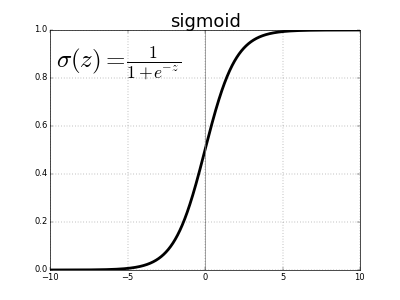
\includegraphics[width=5cm]{images/sigmoid_graph}}
		\caption[Sigmoïde graphique]{Sigmoïde}
		\label{fig:sigmoid-graph}
	\end{wrapfigure} 
	La forme de la fonction pour toutes les entrées possibles est une forme en S de zéro jusqu'à 0,5 à 1,0. Pendant longtemps, jusqu'au début des années 1990, c'était l'activation par défaut utilisée sur les réseaux de neurones \cite{krizhevsky2012imagenet}.
	
	
	
	
	%\begin{figure}[H]%bth
	%	\centering
	%	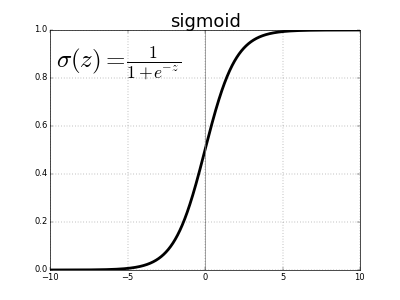
\includegraphics[width=6cm]{images/sigmoid_graph}
	%	\caption{Fonction d'activation sigmoïde, graphique}
	%	\label{fig:sigmoid-graph}
	%\end{figure}

	
	Supposons que $z$ est une fonction linéaire (comme la droite de la formule \ref{eq:droite_sep}). Et la fonction sigmoïde (en partant de la fonction logistique générale, formule \ref{eq:sigmoid-dev}) est :
	\begin{equation}\label{eq:sigmoid-activation}
	{\displaystyle \sigma (z)= {\frac {1}{1+e^{-z}}} ={\frac {1}{1+e^{-(w _{1}x_{1}+\cdots +w_{n}x_{n}+b)}}}}
	\end{equation} 
	
	avec $z = w _{1}x_{1}+\cdots +w_{n}x_{n}+b$.
	
	
	La fonction \textbf{tangente hyperbolique}, ou \textbf{tanh} en abrégé, est une fonction d'activation non linéaire de forme similaire qui génère des valeurs comprises entre -1,0 et 1,0. À la fin des années 1990 et au cours des années 2000, la fonction tanh a été préférée à la fonction d'activation sigmoïde car les modèles qui l'utilisaient étaient plus faciles à entraîner et avaient souvent de meilleures performances prédictives \cite{goodfellow2016deep}.
	La fonction d'activation tangente hyperbolique fonctionne généralement mieux que la sigmoïde logistique.
	
	%\subsubsection*{\qquad \textbullet \ \ Limitations des fonctions d'activation sigmoïde et tanh}
	%Cela signifie que pour tanh et sigmoïde, les grandes valeurs sont alignées sur 1,0 et les petites valeurs sont alignées sur -1 ou 0. De plus, la fonction n'est vraiment sensible qu'aux changements proches du point médian de l'entrée. Par exemple, 0,5 pour les sigmoïdes et 0,0 pour la tanh.
	
	%Les unités sigmoïdales saturent sur la majeure partie de leur domaine - elles saturent à une valeur élevée lorsque z est très positif, saturent à une valeur faible lorsque z est très négatif et ne sont fortement sensibles à leur entrée que lorsque z est proche de 0 \cite{ml2008python}.
	
	%La sensibilité et la saturation limitées de la fonction se produisent indépendamment du fait que l'activation additionnée du nœud fourni en entrée contient des informations utiles ou non. Une fois saturé, il devient difficile pour l'algorithme d'apprentissage de continuer à adapter les poids pour améliorer les performances du modèle \cite{goodfellow2016deep}.\\
	%Les couches profondes des grands réseaux utilisant ces fonctions d'activation non linéaires ne reçoivent pas d'informations de gradient utiles. L'erreur est rétropropagée (voir le chapitre \ref{chap:methode}, section \ref{sec:backprop}) sur le réseau et utilisée pour mettre à jour les pondérations. La quantité d'erreur diminue considérablement avec chaque couche supplémentaire à travers laquelle elle se propage, compte tenu de la dérivée de la fonction d'activation choisie. C'est ce qu'on appelle le problème du gradient de fuite et empêche les réseaux profonds (multicouches) d'apprendre efficacement \cite{geron2017hands}.
	
	%Bien que l'utilisation de fonctions d'activation non linéaires permette aux réseaux de neurones d'apprendre des fonctions de cartographie complexes, elles empêchent efficacement l'algorithme d'apprentissage de fonctionner avec des réseaux profonds.
	
	
	
	\subsubsection{Fonction d'activation ReLU}\label{subsec:relu}
	
	Dans le domaine des réseaux de neurones artificiels, ReLU (Rectified Linear Unit) ou fonction d'activation d'unité linéaire rectifiée est une fonction d'activation définie comme la partie positive de son argument \cite{goodfellow2016deep}.
	$${\displaystyle f(x)=x^{+}=\max(0,x)}$$
	%ReLU signifie fonction d'activation d'unité linéaire rectifiée; c'est une fonction linéaire par morceaux qui produira l'entrée si elle est positive; sinon, la sortie est nulle.
	ReLU est une fonction linéaire par morceaux qui produira l'entrée directement si elle est positive, sinon, la sortie est nulle \cite{tammina2019transfer}. C'est devenu la fonction d'activation par défaut pour de nombreux types de réseaux de neurones, car un modèle qui l'utilise est plus facile à former et atteint souvent de meilleures performances \cite{geron2017hands}.
	
	\begin{wrapfigure}{r}{0.3\textwidth}
		\myfloatalign{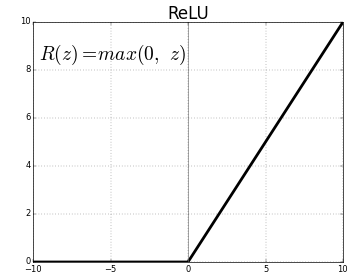
\includegraphics[width=5cm]{images/relu_activation}}
		\caption{ReLU}\label{fig:relu}
	\end{wrapfigure}
	
	La conception d'unités cachées est un domaine de recherche extrêmement actif et ne dispose pas encore de nombreux principes directeurs théoriques définitifs.
	Les fonctions d'activations ReLU sont un excellent choix par défaut d'unité cachée.\\De nombreux autres types d'unités cachées sont disponibles. Il peut être difficile de déterminer quand utiliser quel type, bien que les unités linéaires rectifiées soient généralement un choix acceptable \cite{goodfellow2016deep}. ReLU peut résoudre le problème des gradients de fuite, consultez le didacticiel \cite{pretorius2018critical}.
	
	\subsubsection{Autres fonctions d'activations}
	
	\begin{figure}[H]%bth
		\centering
		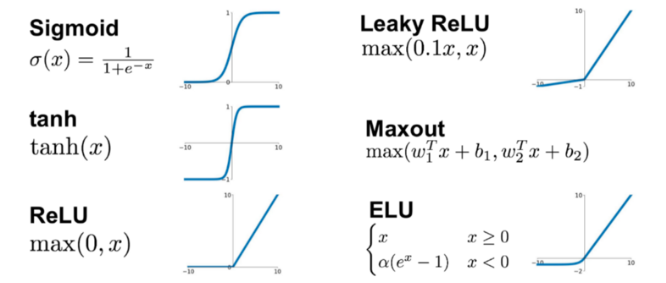
\includegraphics[width=12cm]{images/activation_functions.png}
		\caption{Les différentes fonctions d'activation avec leurs graphes}
		\label{fig:all_activation_function}
	\end{figure}
	
	
	%	\subsection{Neurones}
	%\lipsum[1]
	%\subsubsection{Réseau des neurones}
	
	\subsection{Réseau neuronal convolutif (CNN)}\label{sec:cnn}
	
	Le réseau neuronal convolutif est un type de réseau neuronal artificiel (CNN, Convolutional Neural Network ou ConvNet) qui utilise plusieurs perceptrons qui analysent les entrées d'image et ont des poids et des bases apprenables sur plusieurs parties d'images et capables de se séparer les unes des autres \cite{tammina2019transfer}.
	
	\begin{figure}[H]%bth
		\centering
		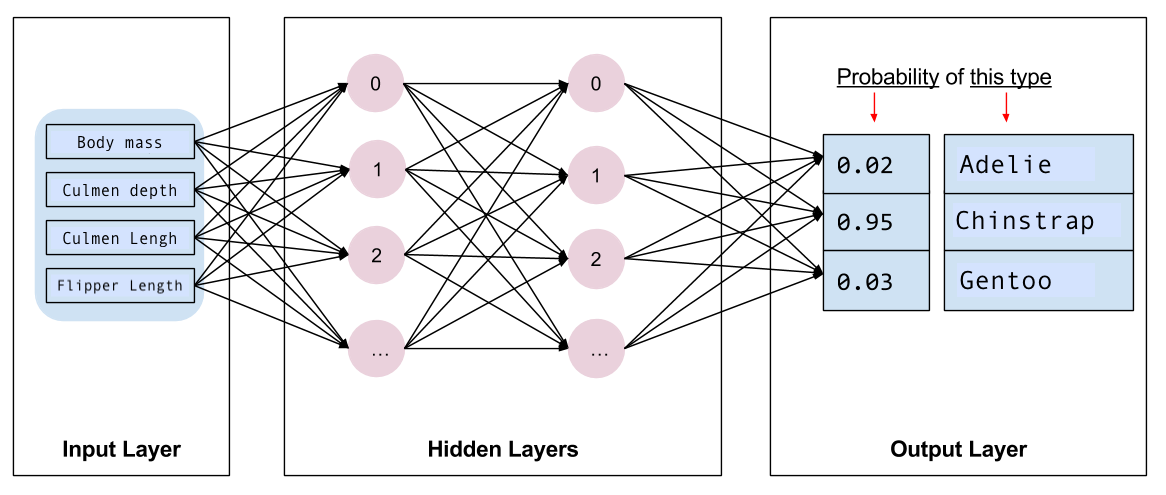
\includegraphics[width=\textwidth]{images/tensorflow_neuron_layer}
		\caption[Exemple de la classification avec un CNN a différentes couches]{Exemple de la classification avec un CNN à différentes couches: la couche d'entrée, les couches cachées et la couche de sortie (respectivement en anglais : Input Layer, Hidden Layers and Output Layer) \cite{ml2008python}}.
		\label{fig:cnn_layers}
	\end{figure}
	
	Le CNN est un type de réseau de neurones acyclique à propagation avant, dans lequel le motif de connexion entre les neurones est inspiré par le cortex visuel des animaux. Les neurones de cette région du cerveau sont arrangés de sorte à ce qu'ils correspondent à des régions (appelés champs réceptifs) qui se chevauchent lors du pavage du champ visuel. Ils sont de plus organisés de manière hiérarchique, en couches (aire visuelle primaire V1, secondaire V2, puis aires V3, V4, V5 et V6, gyrus temporal inférieur), chacune des couches étant spécialisée dans une tâche, de plus en plus abstraite \cite{antoine2018apprentissage}. En simplifiant à l'extrême, une fois que les signaux lumineux sont reçus par la rétine et convertis en potentiels d'action:
	\begin{itemize}
		\item L'aire primaire V1 s'intéresse principalement à la détection de contours, ces contours étant définis comme des zones de fort contraste de signaux visuels reçus.
		\item L'aire V2 reçoit les informations de V1 et extrait des informations telles que la fréquence spatiale, l'orientation, ou encore la couleur.
		\item L'aire V4, qui reçoit des informations de V2, mais aussi de V1 directement, détecte des caractéristiques plus complexes et abstraites liées par exemple à la forme.
		\item Le gyrus temporal inférieur est chargé de la partie sémantique (reconnaissance des objets), à partir des informations reçues des aires précédentes et d'une mémoire des informations stockées sur des objets.
	\end{itemize}
	
	L'architecture et le fonctionnement des réseaux convolutifs sont inspirés par ces processus biologiques. Ces réseaux consistent en un empilage multicouche de perceptrons \cite{tammina2019transfer}, dont le but est de pré-traiter de petites quantités d'informations.\\
	Un réseau convolutif se compose de deux types de neurones, agencés en couches traitant successivement l'information. Dans le cas du traitement de données de type images \cite{antoine2018apprentissage}, on a ainsi : 
	
	\begin{itemize}
		\item des neurones de traitement, qui traitent une portion limitée de l'image (le champ réceptif) au travers d'une fonction de convolution\cite{tammina2019transfer, antoine2018apprentissage};
		\item des neurones de mise en commun des sorties dits d'agrégation totale ou partielle (pooling) \cite{tammina2019transfer, antoine2018apprentissage}.
		
	\end{itemize}

	
	Un traitement correctif non linéaire est appliqué entre chaque couche pour améliorer la pertinence du résultat. L'ensemble des sorties d'une couche de traitement permet de reconstituer une image intermédiaire, dite carte de caractéristiques (feature map), qui sert de base à la couche suivante. Les couches et leurs connexions apprennent des niveaux d'abstraction croissants et extraient des caractéristiques de plus en plus haut niveau des données d'entrée \cite{antoine2018apprentissage, shin2016deep}.
	
	L'un des avantages de l'utilisation du réseau de neurones convolutifs est qu'il exploite l'utilisation de la cohérence spatiale locale dans les images d'entrée, ce qui leur permet d'avoir moins de poids car certains paramètres sont partagés \cite{tammina2019transfer}.
	
	
	\begin{figure}[H]%bth
		\centering
		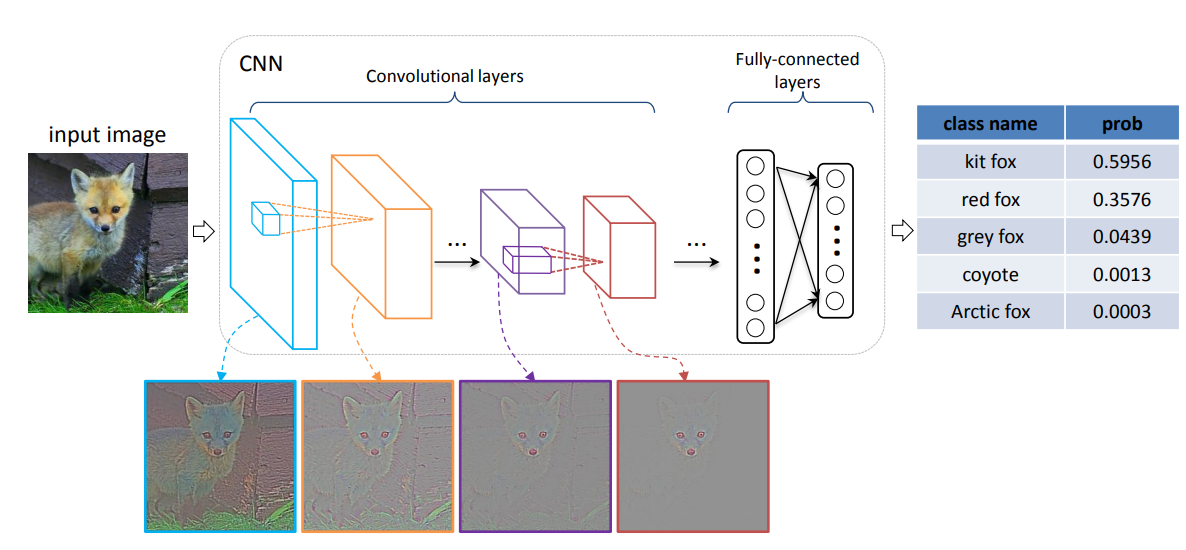
\includegraphics[width=\textwidth]{images/cnn-fox}
		\caption[L'illustration du comportement externe et interne d'un CNN.]{L'illustration du comportement externe et interne d'un CNN. Le comportement externe correspond aux catégories de prédiction de sortie pour les images d'entrée. Le comportement interne est à sonder en visualisant les espaces de représentation construits par chaque couche et les informations visuelles conservées dans chaque couche. \cite{yu2016visualizing}}
		\label{fig:cnn_exemple}
	\end{figure}
	
	
	%\subsubsection{\textbf{Les différents couches d'un CNN}}
	
	\subsubsection{\qquad \textbullet \ \ Couche de convolution}
	
	La couche de convolution est la pierre angulaire du CNN. Il porte la majeure partie de la charge de calcul du réseau.
	
	Cette couche effectue un produit scalaire entre deux matrices, où une matrice est l'ensemble de paramètres apprenables autrement connu sous le nom de noyau (en anglais kernel) $K$ ou encore filtre de convolution, et l'autre matrice est la partie restreinte du champ récepteur $I$. Le noyau est spatialement plus petit qu'une image mais il est plus en profondeur. Cela signifie que, si l'image est composée de trois canaux (RVB), la hauteur et la largeur du noyau seront spatialement petites, mais la profondeur s'étend jusqu'aux trois canaux \cite{goodfellow2016deep}.
	
	\paragraph*{Définition:}
	
	\textit{Soient $h_1, \ h_2 \in \mathbb{N}, {K} \in \mathbb{R}^{(2h_1+1)\times(2h_2+1)}$. 
	La convolution de $I$ par $K$ est donnée par :} 
	\begin{equation} \label{eq:kernel}
		(I\ast K)_{r,s} = \sum_{u=-h_1}^{h_1} \sum_{v=-h_2}^{h_2} K_{u,v}I_{r+u,s+v}
	\end{equation} 
	où $K$ est donnés par : 
	
	$$ 
	K = \begin{bmatrix}
		{K_{-h_1,-h_2}}&\cdots &{K_{-h_1,h_2}}\\
		\vdots &{K_{0,0}} &\vdots \\
		{K_{h_1,-h_2}}&\cdots &{K_{h_1,h_2}}
	\end{bmatrix}
	$$
	
	La taille du filtre $(2h_1+1)\times(2h_2+1)$ précises le champ visuel capturé et traité par $K$.
	Lorsque $K$ parcourt $I$, le déplacement du filtre est réglé par deux paramètres de \textit{stride} (horizontal et vertical). Un stride de 1 horizontal (respectivement vertical) signifie que $K$ se déplace d'une position horizontale (resp. verticale) à chaque application de la formule \ref{eq:kernel}. Les valeurs de stride peuvent également être supérieures et ainsi sous-échantillonner $I$ \cite{goodfellow2016deep, antoine2018apprentissage}.\\
	Le comportement du filtre sur les bords de $I$ doit également être précisé, par l'intermédiaire d'un paramètre de \textit{padding}. Si l'image convoluée $(I\ast K)$ doit posséder la même taille que $I$, alors $2h_{1}$ lignes de 0 ($h_1$ à gauche et $2h_{1}$ à droite) et $2h_{2}$ colonnes de $0$ ($h_2$ en haut et $h_2$ en bas) doivent être ajoutées. Dans le cas où la convolution est réalisée sans padding, l'image convoluée est de taille $n_{1} - 2h_{1} \times n_{2} - 2h_{2}$ \cite{antoine2018apprentissage}.
	
	%\begin{figure}[H]%bth
		%\centering
		%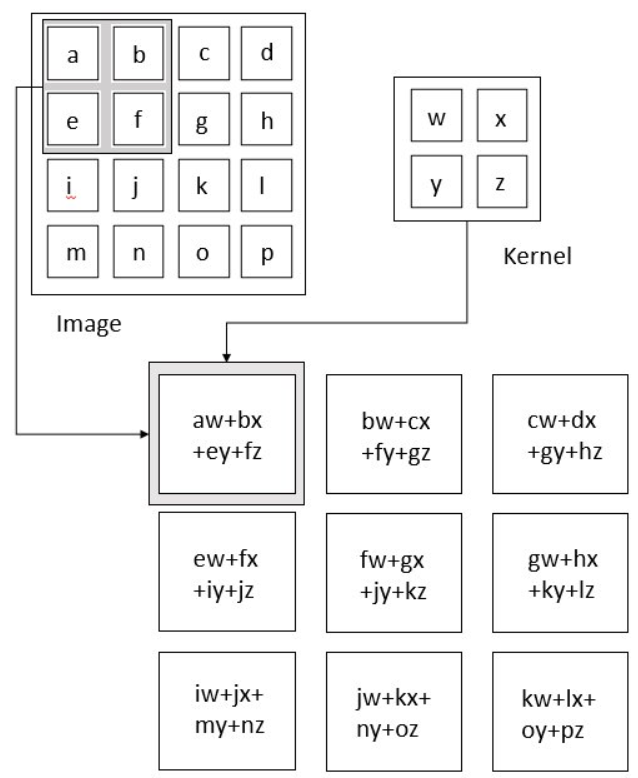
\includegraphics[width=0.4\textwidth]{images/cnn_kernel}
		%\caption[Illustration des calculs effectués dans une opération de convolution.]{Illustration de l'opération de convolution.}
	%	\label{fig:cnn_kernel}
	%\end{figure}
	
		
	
	%\begin{figure}[H]%bth
		%\centering
		%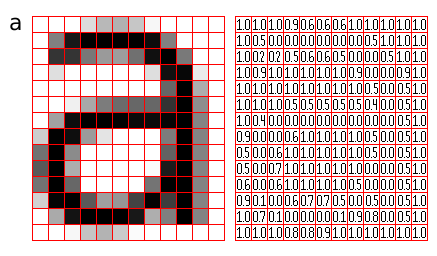
\includegraphics[width=\textwidth]{images/image_pixel}
		%\caption[Représentation de l'image sous forme de grille de pixels.]{Représentation de l'image sous forme de grille de pixels. Il contient une série de pixels disposés en forme de grille qui contient des valeurs de pixel pour indiquer la luminosité et la couleur de chaque pixel.}
		%\label{fig:image_pixel}
	%\end{figure}

	\begin{figure}[H]%bth
		\centering
		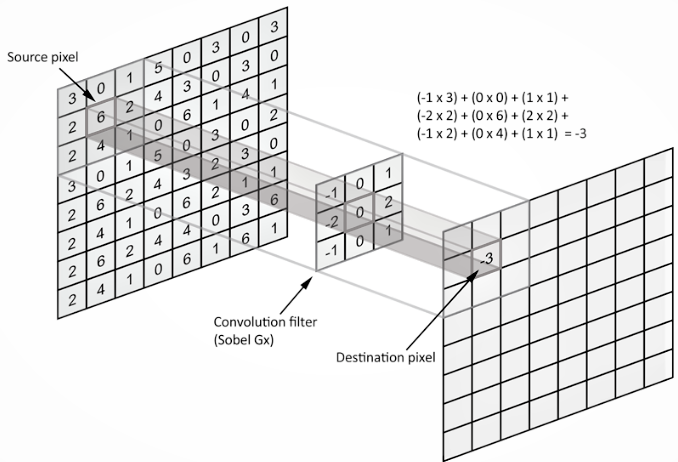
\includegraphics[width=0.8\textwidth]{images/cnn_kernel_filter}
		\caption[Illustration des calculs effectués dans une opération de convolution.]{Illustration des calculs effectués dans une opération de convolution \cite{antoine2018apprentissage}.}
		\label{fig:cnn_kernel_filter}
	\end{figure}
	%Soit $l$ une couche de convolution. L'entrée de la couche $l$ est composée de $n ^ {(l - 1)}$ cartes provenant de la couche précédente, de taille $n_{1} ^ {(l - 1)} * n_{2} ^ {(l - 1)}$. Dans le cas de la rétine $(l = 1)$ l'entrée est l'image $I$. La sortie de la couche $l$ est formée de $n ^ {(l)}$ cartes de taille $n_1 ^ {(l)} \times n_2 ^ {(l)}$. La $i^e$ cartes de la couche $l$ notée $Y_{i} ^ {(l)}$ se calcule comme:
	
	%\begin{equation}
	%	\qquad	Y_i ^ {(l)} =B_i ^ {(l)} + \sum_{j=1}^{n^{(l-1)}} K_{i,j}^{(l)} \ast Y_j^{(l-1)}
	%\end{equation}
	
	%où $B^{()}$ est une matrice de biais et $K_{i,j}^{(l)}$ est le filtre de taille $(2h_1^{(l)}+1)\times(2h_2^{(l)}+1)$ connectant la $j^e$ carte de la couche $(l-1)$ à la $i^e$ carte de la couche $l$.
	
	%$n_{1} ^ {(l)} $ et $ n_{2} ^ {(l)}$ doivent prendre en compte les effets de bords: lors du calcul de la convolution, seuls les pixels dont la somme est définie avec des indices positifs doivent être traités. Dans le cas où le padding n'est pas utilisé, les cartes de sortie ont donc une taille de $n_{1} ^ {(l)} = n_{1} ^ {(l-1)} - 2h_1 ^ {(l)} $ et $ n_{2} ^ {(l)} = n_{2} ^ {(l-1)} - 2h_2 ^ {(l)}$.
	
	Par conséquent, la couche de convolution prend plusieurs images en entrée  et utilise chaque filtre pour calculer la convolution de  chaque image. Le filtre correspond exactement à la caractéristique que nous voulons trouver dans l'image \cite{shin2016deep}. 
	Pour chaque paire (image, filtre), obtenez une carte d'activation ou une carte d'entités montrant où se trouvent les entités dans l'image. Plus la valeur est élevée, plus les points correspondants dans l'image sont similaires à l'entité \cite{goodfellow2016deep}.
	
	%Souvent, les filtres utilisés pour calculer $Y_i ^ {(l)}$ sont les mêmes. De plus, la somme dans l'équation (10.3) peut être conduite sur un sous ensemble des cartes d'entrée.
	
	
		
	\subsubsection{\textbf{L'architecture VGGNet}}\label{subsec:vggnet}
	
	VGG signifie Visual Geometry Group, il s'agit d'une architecture standard de réseau de neurones à convolution profonde (CNN) à plusieurs couches \cite{simonyan2014very}. %Le "profond" fait référence au nombre de couches avec VGG-16 ou VGG-19 composé de 16 et 19 couches convolutionnelles.
	
	Les réseaux VGG ont été les premiers à utiliser de petits filtres de convolution (3×3) et à les combiner pour décrire des séquences de convolution, l'idée étant d'émuler l'effet de larges champs réceptifs par cette séquence. Cette technique amène malheureusement à un nombre exponentiel de paramètres (le modèle entraîné qui peut être téléchargé a une taille de plus de 500 Mo). VGG a concouru à ILSVRC 2014, a obtenu un taux de bonne classification de 92.3\% mais n'a pas remporté le concours \cite{krizhevsky2012imagenet}. Aujourd'hui, VGG est une famille de réseaux profonds (de A à E) qui varient par leur architecture (figure \ref{fig:VGG16_model}). %Le nombre de paramètres (en millions) pour les réseaux de A à E est 133, 133, 134, 138 et 144. Les réseaux VGG-D et VGG-E sont les plus précis et populaires.???
	
	L'architecture VGG est  la base d'un modèle innovant de reconnaissance d'objets. Développé en tant que réseau neuronal profond, VGGNet va au-delà d'ImageNet et dépasse la ligne de base  de nombreuses tâches et ensembles de données. De plus, c'est toujours l'une des architectures de reconnaissance d'images les plus populaires \cite{tammina2019transfer, antoine2018apprentissage}.
	
	Les VGGNet sont basés sur les caractéristiques les plus essentielles des réseaux de neurones convolutifs (CNN). Le graphique suivant montre le concept de base du fonctionnement d'un CNN.
	
	
	\begin{list}{--}{Un bref coup d'œil à l'architecture de VGG :}
		\item \textbf{Entrée} : Le VGGNet prend une taille d'entrée d'image de 224×224. Pour le concours ImageNet, les créateurs du modèle ont recadré le patch central 224 × 224 dans chaque image pour conserver la cohérence de la taille d'entrée de l'image \cite{simonyan2014very}.
		
		\item \textbf{Couches convolutives }: Les couches convolutives de VGG tirent parti d'un champ de réception minimal, c'est-à-dire 3 × 3, la plus petite taille possible qui capture toujours haut/bas et gauche/droite. De plus, il existe également des filtres de convolution 1 × 1 agissant comme une transformation linéaire de l'entrée. Vient ensuite une unité ReLU, qui est une énorme innovation d'AlexNet qui réduit le temps de formation. La foulée de convolution est fixée à 1 pixel pour conserver la résolution spatiale préservée après la convolution (la foulée est le nombre de décalages de pixels sur la matrice d'entrée) \cite{krizhevsky2012imagenet,tammina2019transfer}.
		
		\item \textbf{Couches cachées} : Toutes les couches cachées du réseau VGG utilisent ReLU. VGG n'utilise généralement pas la normalisation de la réponse locale (LRN) car elle augmente la consommation de mémoire et le temps de formation. De plus, il n'apporte aucune amélioration à la précision globale \cite{tammina2019transfer}.
		
		\item \textbf{Couches entièrement connectées} : Le VGGNet a trois couches entièrement connectées. Sur les trois couches, les deux premières ont 4096 canaux chacune et la troisième a 1000 canaux, 1 pour chaque classe \cite{tammina2019transfer}.
		
	\end{list}
	%------------------------------------------------------------------------------
	%\cite{simonyan2014very}
	%\cite{shin2016deep} 
	%\cite[ReLU]{pretorius2018critical}
	%------------------------------------------------------------------------------
	
	
	\begin{figure}[H]%bth
		\centering
		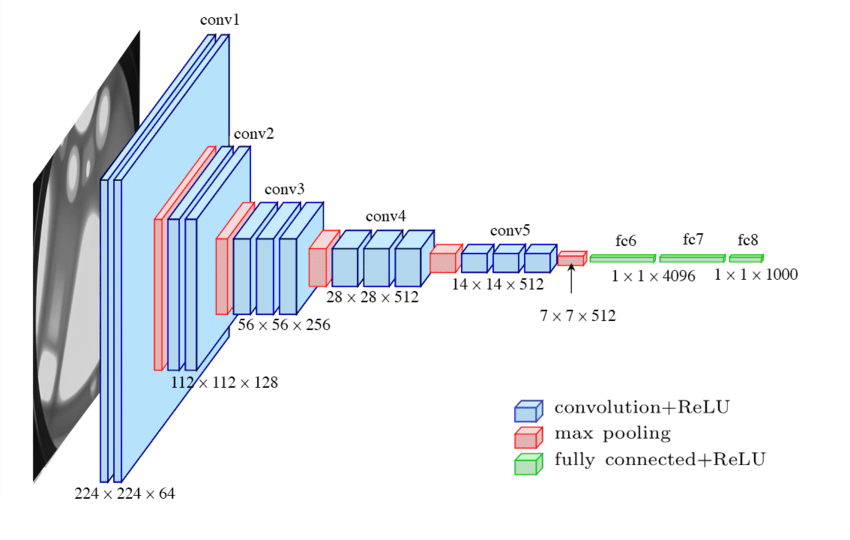
\includegraphics[width=\textwidth]{images/VGG-16-network-architecture.png}
		\caption{CNN : architecture VGG \cite{ml2008python}}.
		\label{fig:VGG_network}
	\end{figure}

	\paragraph{Le modèle VGG16 et VGG19 :}
	
	Visual Geometry Group et se compose de blocs, où chaque bloc est composé de couches 2D Convolution et Max Pooling. Il se décline en deux modèles - VGG16 et VGG19 - avec 16 et 19 couches \cite{yu2016visualizing}.
	
	\textbf{VGG16} (également VGGNet-16) est modèle VGGNet, qui prend en charge 16 couches convolutives.
	Le nombre de filtres que nous pouvons utiliser double à chaque étape ou à travers chaque pile de la couche de convolution. C'est un principe majeur utilisé pour concevoir l'architecture du réseau VGG16. L'un des principaux inconvénients du réseau VGG16 est qu'il s'agit d'un réseau énorme, ce qui signifie qu'il faut plus de temps pour former ses paramètres \cite{yu2016visualizing}.\\
	En raison de sa profondeur et du nombre de couches entièrement connectées, le modèle VGG16 fait plus de 533 Mo. Cela rend la mise en œuvre d'un réseau VGG une tâche fastidieuse.\\
	Le modèle VGG16 est utilisé dans plusieurs problèmes de classification d'images d'apprentissage en profondeur, mais des architectures de réseau plus petites telles que GoogLeNet et SqueezeNet sont souvent préférables. Dans tous les cas, le VGGNet est un excellent élément de base à des fins d'apprentissage car il est simple à mettre en œuvre.
	
	%VGG16 surpasse largement les versions précédentes des modèles des compétitions ILSVRC-2012 et ILSVRC-2013. De plus, le résultat VGG16 est en compétition pour le vainqueur de la tâche de classification (GoogLeNet avec une erreur de 6,7\%) et surpasse considérablement la soumission gagnante ILSVRC-2013 Clarifai. Il a obtenu 11,2\% avec des données de formation externes et environ 11,7\% sans elles. En termes de performances à réseau unique, le modèle VGGNet-16 obtient le meilleur résultat avec environ 7,0\% d'erreur de test, dépassant ainsi un seul GoogLeNet d'environ 0,9\% \cite{simonyan2014very}.
	
	\begin{figure}[H]%bth
		\centering
		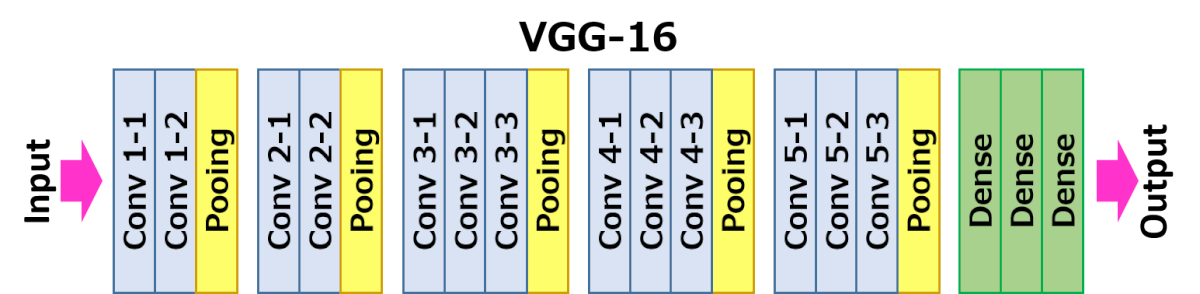
\includegraphics[width=\textwidth]{images/vgg16.png}
		\caption{Le modèle VGG-16 \cite{tammina2019transfer}}
		\label{fig:VGG16_model}
	\end{figure}

	Le concept du modèle \textbf{VGG19} (également VGGNet-19) est le même que celui du VGG16, sauf qu'il prend en charge 19 couches. Le « 16 » et le « 19 » représentent le nombre de couches de poids dans le modèle (couches convolutives). Cela signifie que VGG19 a trois couches convolutionnelles de plus que VGG16. Nous aborderons plus en détail les caractéristiques des réseaux VGG16 et VGG19 dans la dernière partie de cet article \cite{yu2016visualizing}.


	
	%\subsubsection{Réseau neuronal récurrent (RNN)}
	%\lipsum[1]
	
	%\section{Réseaux de neurones}
	
	
	
	%\section{Classificateurs}
	%\lipsum[1]


